\Chapter{Adatok egységes struktúrába szervezése}

Ebben a fejezetben a vizsgált adathalmazok egységes adatstruktúrába szervezésének folyamata kerül bemutatásra. A fejezet célja annak ismertetése, hogy a korábban elkülönítve feldolgozott, eltérő szerkezetű adatkészletek hogyan alakíthatók át egy közös, jól strukturált adatsémává, amely alkalmas további elemzési és gépi tanulási feladatok elvégzésére.

A fejezet első részében az adathalmazok közötti kapcsolatok és relációs sémák elemzése történik meg, amely alapot szolgáltat az adatok logikus felépítéséhez. Ezt követően bemutatásra kerülnek az alkalmazott normalizálási lépések, valamint azok indoklása az adatbázis-tervezési alapelvek figyelembevételével. A továbbiakban az adatok tisztításával kapcsolatos feladatok kerülnek ismertetésre, különös tekintettel a hiányzó és inkonzisztens értékek kezelésére. A fejezet zárásaként az egyes adathalmazok összevonásának (merge) folyamata kerül bemutatásra, amelynek eredményeként egy egységes, elemzésre kész adatstruktúra jön létre.

\Section{Relációs sémák elemzése}

Az adathalmazok egységes struktúrába szervezésének első lépéseként az egyes adatkészletek relációs sémáinak elemzése történt meg. A vizsgálat célja az volt, hogy feltárja az adatok belső szerkezetét, az attribútumok közötti kapcsolatokat, valamint azokat az azonosítókat, amelyek az adathalmazok későbbi összekapcsolását lehetővé teszik.

A feldolgozás során az A, B és C adathalmazokhoz külön relációs sémák kerültek kialakításra. Ezek a sémák az egyes adatkészletek logikai felépítését írják le, kiemelve a fő entitásokat, azok attribútumait, valamint az elsődleges és idegen kulcsokat. Az elkülönített sémák vizsgálata lehetővé tette az adathalmazok közötti hasonlóságok és szerkezeti eltérések azonosítását.

Az A adathalmaz relációs sémája a videojátékok alapvető jellemzőit tartalmazza, és referenciapontként szolgált a további adatkészletek integrálása során. A B és C adathalmazok sémái kiegészítő információkat hordoznak, amelyek eltérő attribútumkészlettel rendelkeznek, ugyanakkor közös játékazonosítók mentén kapcsolhatók az A adathalmazhoz.

Az A, B és C adathalmazok sémáinak elemzését követően került kialakításra a D adathalmaz relációs sémája, amely az eredeti adatkészletek összevonásával létrehozott, egységes adatstruktúrát írja le. A D adathalmaz sémája már a normalizálási és tisztítási lépések eredményét tükrözi, és közvetlen alapját képezi a további elemzési és gépi tanulási feladatoknak.

A sémák elemzése során meghatározásra került az adathalmazok összevonásának prioritási sorrendje is. Az integrálás során a C adathalmaz szolgált elsődleges adatforrásként, mivel ez tartalmazta a legfrissebb információkat. A B, majd az A adathalmaz adatai kiegészítő jelleggel kerültek figyelembevételre, elsősorban azon attribútumok esetében, amelyek a C adathalmazban nem, vagy csak hiányosan álltak rendelkezésre. Ez a prioritási sorrend biztosította, hogy az összevont adathalmaz a lehető legaktuálisabb adatokat tükrözze.

A relációs sémák vizsgálata rávilágított arra, hogy az eltérő szerkezetű adathalmazok integrálása csak előzetes normalizálási és adatelőkészítési lépések után valósítható meg hatékonyan. A feltárt kapcsolatok és függőségek szolgáltak alapul a következő alfejezetben bemutatott normalizálási folyamatokhoz, valamint az adathalmazok összevonásának megvalósításához.

\Section{Normalizálás}

A normalizálás célja az adatredundancia csökkentése, az adatintegritás biztosítása, valamint az adatok logikus, karbantartható és bővíthető szerkezetbe rendezése. A dolgozat során alkalmazott normalizálási lépések az első, második és harmadik normálforma (1NF–3NF) követelményeit követik, figyelembe véve az egyes adathalmazok eltérő szerkezeti sajátosságait.

\subsection{Az A adathalmaz normalizálása}

\subsubsection{Első normálforma (1NF)}

Az eredeti CSV állomány több olyan attribútumot tartalmazott, amelyek nem atomi értékeket vettek fel. Ilyenek voltak például a több elemet tartalmazó címkék, műfajok, kategóriák, platformok, valamint a képernyőképeket és videókat leíró mezők. Az első normálforma követelménye szerint minden attribútumnak oszthatatlan, atomi értéket kell tartalmaznia, ezért ezek az összetett és listaértékű attribútumok külön táblákba kerültek.

A listaértékű adatok kezelésére külön entitások és kapcsolótáblák kerültek kialakításra. A címkék, műfajok, platformok és kategóriák önálló táblákban kerültek tárolásra, míg a játékok és ezen attribútumok közötti több–több kapcsolatokat kapcsolótáblák reprezentálják. Az A adathalmazban a címkék eredetileg több különálló oszlopban szerepeltek, amelyek a feldolgozás során egységes szerkezetbe kerültek összevonásra, és egy szótárjellegű (dictionary) struktúrában lettek eltárolva a további normalizálási lépések megkönnyítése érdekében. 

A médiatartalmak – képernyőképek és videók – esetében minden egyes elem külön rekordként került eltárolásra. A képernyőképeket tartalmazó attribútumok további bontása is szükségessé vált, mivel az eredeti adathalmaz teljes méretű és előnézeti képeket egyetlen struktúrában tárolt. Ennek megfelelően a képernyőképek külön attribútumokra kerültek bontásra a teljes felbontású (\textit{screenshots\_full}) és az előnézeti (\textit{screenshots\_thumbs}) képek elkülönített kezelésére. Hasonló módon a videók esetében külön attribútumok kerültek kialakításra az eltérő típusú és felbontású médiaforrások kezelésére (\textit{movies\_thumbnail}, \textit{movies\_max}, \textit{movies\_480}). A rendszerkövetelmények szintén felbontásra kerültek operációs rendszer és követelménytípus (minimum, ajánlott) szerint. 

A rendszerkövetelmények esetében az eredeti, platformonként elkülönített mezők egységes struktúrába kerültek átszervezésre, ahol az operációs rendszer (\textit{windows}, \textit{mac}, \textit{linux}) külön attribútumban jelenik meg. A követelmények típusa egy külön \textit{type} mező segítségével került megkülönböztetésre, amely minimum és ajánlott értékeket vehet fel, míg a konkrét hardver- és szoftverkonfiguráció a \textit{requirements} mezőben kerül tárolásra.


\subsubsection{Második normálforma (2NF)}

A második normálforma biztosítása érdekében vizsgálatra kerültek az elsődleges kulcstól való részleges függőségek. Az A adathalmaz központi táblája a \textit{game} entitás, amelynek elsődleges kulcsa az \textit{appid}. Azokat az attribútumokat, amelyek ugyan az \textit{appid}-tól függenek, de nem a játék alapadatait írják le, külön táblákba kerültek szétválasztásra.

Ennek eredményeként önálló táblák jöttek létre a részletes és rövid leírások kezelésére, a támogatási információk (például URL és e-mail cím) tárolására, valamint a médiához kapcsolódó elemek elkülönítésére. A rendszerkövetelmények kezelése szintén külön táblában történt, az operációs rendszer és a követelménytípus figyelembevételével.

\subsubsection{Harmadik normálforma (3NF)}

A harmadik normálforma megvalósítása során a tranzitív függőségek megszüntetésére került sor. A fejlesztők és kiadók adatai önálló entitásokba kerültek, és a játékokhoz kapcsolótáblákon keresztül kapcsolódnak. Ez a megoldás lehetővé tette a redundáns szöveges adatok elkerülését és az adatok konzisztens kezelését. Az adathalmazban szereplő fejlesztőkre és kiadókra vonatkozó attribútumok elnevezései az eredeti struktúrát követték (\textit{developer}, \textit{publisher}), azonban a normalizált sémában ezek önálló entitásokként jelennek meg, biztosítva az egységes elnevezést és a redundanciamentes adatkezelést.

Hasonló módon a kategóriák, műfajok, címkék és platformok esetében is külön táblák tárolják az egyedi értékeket, míg a játékokkal való kapcsolatukat kizárólag azonosítók segítségével megvalósított kapcsolótáblák reprezentálják. A több–több kapcsolatok minden esetben explicit módon, kapcsolótáblák segítségével kerültek kezelésre.

\subsubsection{Összegzés}

A normalizálási folyamat eredményeként az A adathalmaz relációs sémája több, logikailag elkülönülő entitásból épül fel. A központi \textit{game} tábla mellett önálló táblák jöttek létre a leírások, támogatási információk, médiatartalmak, rendszerkövetelmények, valamint a különböző kategorizáló attribútumok kezelésére. A sémában minden több–több kapcsolat külön kapcsolótáblán keresztül valósul meg, biztosítva az adatok redundanciamentes tárolását.

Az A adathalmaz normalizálási lépései biztosították az adatredundancia minimalizálását, a tranzitív függőségek megszüntetését, valamint a listaértékű és összetett attribútumok önálló táblákba történő szétválasztását. A kialakított relációs séma jól strukturált, karbantartható és alkalmas arra, hogy alapjául szolgáljon a további adatintegrációs és gépi tanulási feladatoknak.

Az A adathalmaz részletes attribútumleírását és az egyes mezők jelentését tartalmazó adatleíró (data dictionary) a dolgozat mellékletei között érhető el. Az A adathalmaz normalizálatlan relációs sémáját a \ref{fig:A_unnormalized} ábra, míg a normalizált relációs sémát a
\ref{fig:A_normalized} ábra szemlélteti.


\begin{figure}[H]
    \centering
    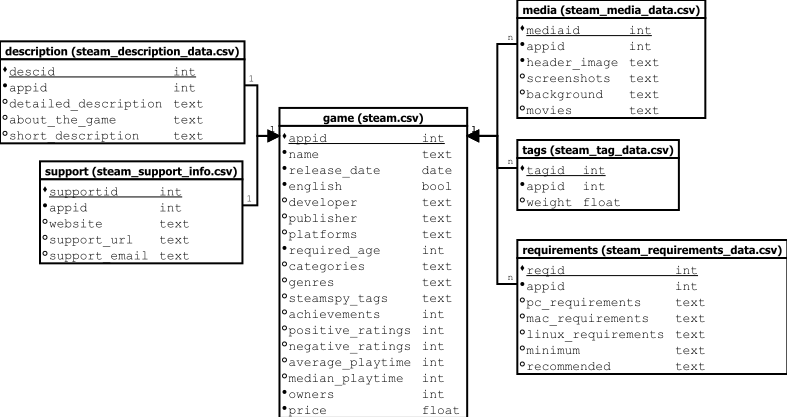
\includegraphics[width=1.0\textwidth]{images/A_unnormalized.pdf}
    \caption{Az A adathalmaz normalizálatlan relációs sémája}
    \label{fig:A_unnormalized}
\end{figure}

\begin{figure}[H]
    \centering
    \includegraphics[width=1.0\textwidth]{images/A_normalized.pdf}
    \caption{Az A adathalmaz normalizált relációs sémája}
    \label{fig:A_normalized}
\end{figure}

\subsection{A B adathalmaz normalizálása}

\subsubsection{Első normálforma (1NF)}

Az eredeti \textit{games.csv} állomány több ismétlődő és listaértékű attribútumot tartalmazott, például képernyőképeket, címkéket, kategóriákat, műfajokat, támogatott nyelveket, szinkronhangokat és játékcsomagokat. Az első normálforma követelményeinek megfelelően ezek az attribútumok felbontásra kerültek, és az adatok atomi értékeket tartalmazó táblákba lettek átszervezve.

A médiatartalmak – képek és videók – külön táblákban kerültek tárolásra, ahol minden elem önálló rekordot képez. A kategóriák, műfajok és címkék esetében önálló entitások jöttek létre, míg a játékokkal való több–több kapcsolatukat kapcsolótáblák reprezentálják. A nyelvek külön táblában kerültek eltárolásra, és a játékokhoz való kapcsolódásuk felirat és szinkronhang szerinti bontásban történt. A platformok kezelése szintén normalizált formában, külön táblák és kapcsolatok segítségével valósult meg.

A játékcsomagok összetett szerkezete miatt többszintű modell került kialakításra, amely elkülöníti a csomag alapadatait és azok alelemeit, biztosítva az adatok áttekinthető és atomi szintű tárolását.

\subsubsection{Második normálforma (2NF)}

A második normálforma biztosítása érdekében a részleges függőségek megszüntetésére került sor. A központi \textit{game} tábla elsődleges kulcsa az \textit{appid}, amelyhez kizárólag a játék alapadatai tartoznak. Azok az attribútumok, amelyek nem közvetlenül a játék leírását szolgálják, külön relációkba kerültek.

Ennek eredményeként önálló táblák jöttek létre a támogatási információk, médiatartalmak, kategorizáló attribútumok, nyelvek, fejlesztők, kiadók, platformok és csomagadatok kezelésére. A több–több kapcsolatok minden esetben asszociatív táblák segítségével kerültek megvalósításra, biztosítva az adatok egyértelmű és redundanciamentes összekapcsolását.

\subsubsection{Harmadik normálforma (3NF)}

A harmadik normálforma megvalósítása során a tranzitív függőségek megszüntetése volt a cél. A címkék, műfajok, nyelvek, fejlesztők, kiadók, kategóriák, platformok és csomagok megnevezései önálló táblákban kerültek eltárolásra, így elkerülhetővé vált a redundáns szöveges adatok ismétlődése.

A nyelvek kezelése egységes módon történt, ahol az egyes nyelvek egyszer kerülnek tárolásra, és külön kapcsolótáblák jelzik, hogy egy adott játék rendelkezik-e feliratokkal vagy hanggal az adott nyelven. Ez a megoldás megszüntette a korábbi listaértékű mezők közötti redundanciát. A játékcsomagok többszintű felépítése szintén a tranzitív függőségek elkerülését és az adatok logikus strukturálását szolgálta.

\subsubsection{Összegzés}

A normalizálás eredményeként a B adathalmaz relációs sémája egy jól strukturált, több entitásból álló adatmodellt alkot. A központi \textit{game} tábla mellett önálló relációk kezelik a támogatási információkat, médiatartalmakat, kategorizáló attribútumokat, nyelveket, fejlesztőket, kiadókat, platformokat, valamint a játékcsomagok és azok al-elemeinek adatait. A séma minden több–több kapcsolatot külön kapcsolótáblákon keresztül valósít meg.

A B adathalmaz normalizálási folyamata eredményeként egy tiszta, jól strukturált adatmodell jött létre, amely megfelel az első három normálforma követelményeinek. A kialakított séma atomi értékeket tartalmaz, megszünteti a részleges és tranzitív függőségeket, valamint külön táblákban kezeli az összetett és listaértékű mezőket. Az alkalmazott struktúra jól bővíthető, karbantartható, és minimális adatredundanciát biztosít a további feldolgozási és elemzési lépésekhez.

A B adathalmaz normalizált sémájához tartozó adatleíró (data dictionary), amely az attribútumok jelentését és típusát részletezi, a dolgozat mellékleteiben található. A B adathalmaz normalizálatlan relációs sémáját a \ref{fig:B_unnormalized} ábra, míg a normalizált relációs sémát a \ref{fig:B_normalized} ábra szemlélteti.

\begin{figure}[H]
    \centering
    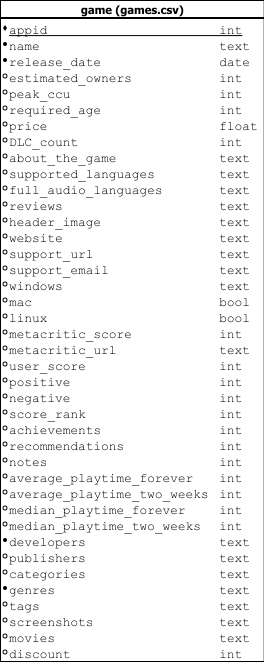
\includegraphics[width=0.6\textwidth]{images/B_unnormalized.pdf}
    \caption{A B adathalmaz normalizálatlan relációs sémája}
    \label{fig:B_unnormalized}
\end{figure}

\begin{figure}[H]
    \centering
    \includegraphics[width=1.0\textwidth]{images/B_normalized.pdf}
    \caption{A B adathalmaz normalizált relációs sémája}
    \label{fig:B_normalized}
\end{figure}

\subsection{A C adathalmaz normalizálása}

A C adathalmaz normalizálásának kiindulópontját négy, időben és feldolgozottságban eltérő CSV-fájl képezte: a 2024 májusi és a 2025 márciusi adatállományok nyers (\textit{full}) és előfeldolgozott (\textit{cleaned}) változatai. A \textit{full} állományok a Steam \cite{steam} áruházból származó teljes, nyers adatokat tartalmazták, míg a \textit{cleaned} változatok már előzetes tisztításon átesett, duplikációktól mentes adatokat biztosítottak.

A 2025-ös adatkészletek a korábbi verziókhoz képest egy további attribútummal is bővültek, amely a játékok aktuális kedvezményét (\textit{discount}) írja le. A normalizálás során az eltérő időpontokból és szerkezetből adódó különbségek egységes kezelése kiemelt szempont volt.

\subsubsection{Első normálforma (1NF)}

Az eredeti CSV-fájlok több olyan attribútumot tartalmaztak, amelyek nem atomi értékeket vettek fel. Ilyenek voltak például a képernyőképek, címkék, kategóriák, műfajok, valamint a támogatott feliratokat és szinkronhangokat tartalmazó mezők. Az első normálforma követelményeinek megfelelően ezek az összetett és listaértékű attribútumok külön relációkba kerültek.

A normalizálás során önálló entitások jöttek létre többek között a médiatartalmak, képernyőképek, videók, leírások, kategóriák, műfajok, nyelvek, platformok és játékcsomagok kezelésére. A nyelvi attribútumok két külön relációban kerültek eltárolásra, megkülönböztetve a feliratokat és a szinkronhangokat. Ez a felosztás lehetővé tette a nyelvi támogatás pontosabb és redundanciamentes kezelését.

\subsubsection{Második normálforma (2NF)}

A második normálforma biztosítása érdekében a részleges függőségek megszüntetésére került sor. A játékokat leíró központi tábla elsődleges kulcsa az \textit{appid}, amelyhez kizárólag a játék alapadatai tartoznak. Azok az attribútumok, amelyek ugyan az \textit{appid}-tól függnek, de nem közvetlenül a játék alapjellemzőit írják le, külön relációkba kerültek.

Önálló táblák jöttek létre többek között a támogatási információk, médiatartalmak, leírások, kategóriák, műfajok, nyelvek, fejlesztők, kiadók, címkék, platformok és játékcsomagok kezelésére. A redundáns szöveges ismétlődések megszüntetésre kerültek azáltal, hogy az egyes entitások megnevezései saját táblákban szerepelnek, míg a játékokkal való kapcsolatukat kizárólag azonosítók biztosítják.

\subsubsection{Harmadik normálforma (3NF)}

A harmadik normálforma megvalósítása során a tranzitív függőségek megszüntetése volt a cél. A kategóriák, műfajok, nyelvek, fejlesztők, kiadók, címkék, platformok és csomagok megnevezései önálló entitásokban kerültek eltárolásra, míg a játékokkal való kapcsolatukat külön asszociatív táblák írják le.

A játékcsomagok kezelése háromszintű struktúrában valósult meg. A játék és a csomag közötti kapcsolatot egy kapcsolótábla reprezentálja, míg a csomagok alapadatai és azok alelemei külön relációkban kerültek eltárolásra. Ez a megoldás biztosítja az összetett csomagstruktúrák áttekinthető és redundanciamentes kezelését.

\subsubsection{Összegzés}

A normalizálás eredményeként a C adathalmaz relációs sémája egy egységes, jól strukturált adatmodellt alkot. A központi \textit{game} tábla mellett önálló relációk kezelik a támogatási információkat, médiatartalmakat, leírásokat, kategorizáló attribútumokat, nyelveket, fejlesztőket, kiadókat, platformokat, valamint a játékcsomagok és azok al-elemeinek adatait. A 2025-ös adatkészletekben megjelenő \textit{discount} attribútum a végső sémában is elkülönítve, konzisztens módon került kezelésre.

A C adathalmaz normalizálása során négy különálló, eltérő időpontból származó CSV-fájl került egységes relációs struktúrába szervezésre. Az alkalmazott normalizálási lépések biztosítják az első három normálforma követelményeinek teljesülését, elkülönítik a felirat- és hangnyelveket, valamint strukturált módon kezelik a játékcsomagokat. A kialakított séma csökkenti az adatredundanciát, elősegíti az adatok konzisztenciáját, és rugalmasan kezeli a 2024-es és 2025-ös adatforrások közötti eltéréseket, így megfelelő alapot biztosít a további integrációs és elemzési feladatokhoz.

A C adathalmaz normalizált sémájához tartozó adatleíró (data dictionary), amely az egyes attribútumok jelentését és típusát részletezi, a dolgozat mellékleteiben található. A C adathalmaz normalizálatlan relációs sémáját a\ref{fig:C_unnormalized} ábra, míg a normalizált relációs sémát a \ref{fig:C_normalized} ábra szemlélteti.

\begin{figure}[H]
    \centering
    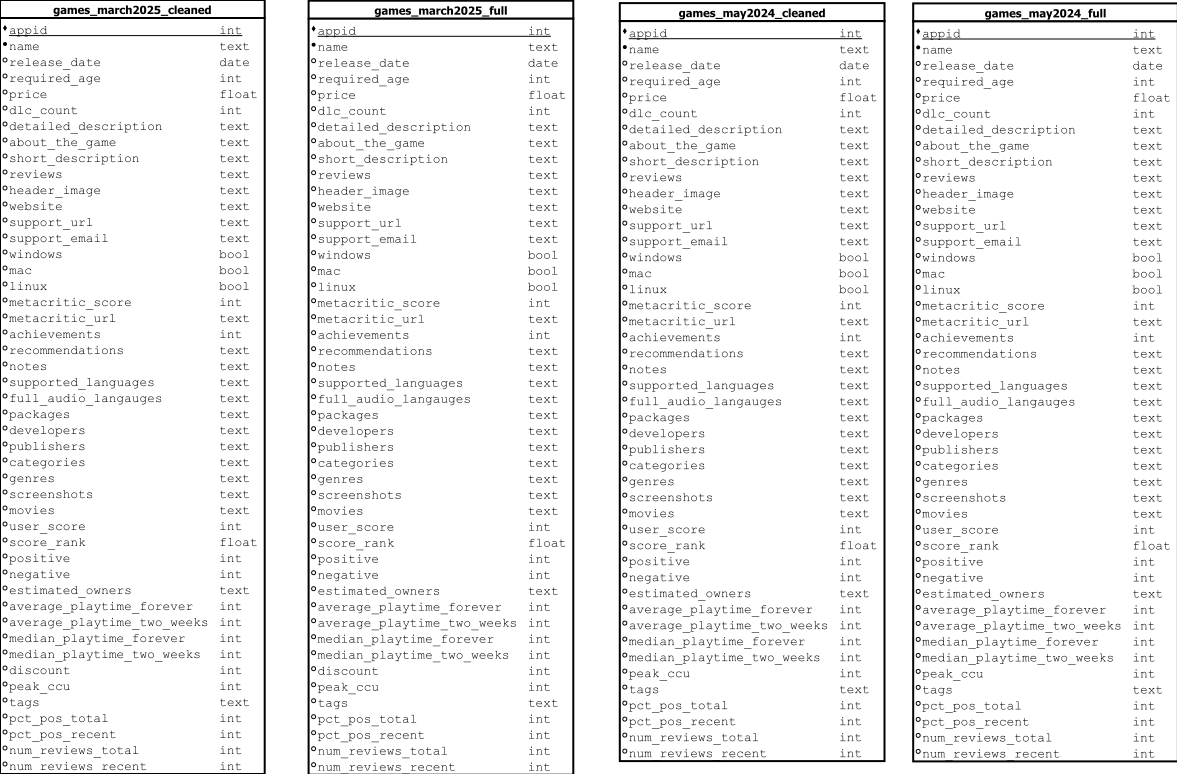
\includegraphics[width=1.0\textwidth]{images/C_unnormalized.pdf}
    \caption{A C adathalmaz normalizálatlan relációs sémája}
    \label{fig:C_unnormalized}
\end{figure}

\begin{figure}[H]
    \centering
    \includegraphics[width=1.0\textwidth]{images/C_normalized.pdf}
    \caption{A C adathalmaz normalizált relációs sémája}
    \label{fig:C_normalized}
\end{figure}

\subsection{A D adathalmaz normalizálása}

A D adathalmaz egységes relációs sémája az A, B és C adathalmazok összevonásával és strukturális egységesítésével jött létre. Kiindulási alapként több, eltérő forrásból származó CSV-fájl szolgált, amelyek részben különböző szerkezettel, eltérő attribútumkészlettel és eltérő időpontokból származó adatokat tartalmaztak. A normalizálás célja egy olyan konzisztens, redundanciamentes adatmodell kialakítása volt, amely egységesen kezeli az eltérő forrásokból származó információkat.

A 2024-es és 2025-ös adatkészletek közötti egyik lényeges eltérés, hogy a 2025-ös verziók egy további attribútumot is tartalmaztak, amely a játékok aktuális kedvezményét (\textit{discount}) írja le. Az egységesítés során ezek a forrásbeli különbségek kezelhető módon kerültek beépítésre a végső sémába.

\subsubsection{Első normálforma (1NF)}

Az összevont CSV-fájlok több olyan attribútumot tartalmaztak, amelyek nem atomi értékeket vettek fel, például címkéket, műfajokat, kategóriákat, támogatott nyelveket, hangnyelveket, csomagstruktúrákat és rendszerkövetelményeket JSON formátumban. Az első normálforma követelményeinek megfelelően ezek az összetett és listaértékű mezők önálló relációkba kerültek.

Az ilyen attribútumok kezelésére külön entitások és kapcsolótáblák jöttek létre, amelyek a játékokkal való kapcsolatot asszociatív módon írják le. Ide tartoznak többek között a felirat és szinkronhangok kezelése, a címkék, műfajok, kategóriák, platformok, valamint a többszintű csomagszerkezetek és a rendszerkövetelmények strukturált tárolása. Ez a felbontás biztosítja, hogy minden attribútum atomi értéket vegyen fel, és megfeleljen az első normálforma előírásainak.

\subsubsection{Második normálforma (2NF)}

A második normálforma megvalósítása érdekében a részleges függőségek megszüntetésére került sor. A D adathalmaz központi táblája a \textit{game} entitás, amelynek elsődleges kulcsa az \textit{appid}. Azok az attribútumok, amelyek az \textit{appid}-tól függnek, de nem a játék alapadatait írják le, külön relációkba kerültek.

Ennek eredményeként önálló táblák jöttek létre többek között a leírások, támogatási információk, médiatartalmak, képernyőképek, videók, rendszerkövetelmények, nyelvek, tulajdonosi tartományok, valamint a csomagok és azok alelemeinek kezelésére. Ez a szétválasztás biztosítja, hogy minden nem kulcsattribútum teljes mértékben függjön az elsődleges kulcstól.

\subsubsection{Harmadik normálforma (3NF)}

A harmadik normálforma teljesítése érdekében a tranzitív függőségek megszüntetésre kerültek. Az ismétlődő szöveges attribútumok – például címkék, műfajok, kategóriák, nyelvek, platformok, fejlesztők és kiadók – önálló entitásokban kerültek eltárolásra, míg a játékokkal való kapcsolatukat külön asszociatív táblák reprezentálják.

A több-több kapcsolatok minden esetben kapcsolótáblák segítségével kerülnek kezelésre, biztosítva az adatok konzisztenciáját és a redundancia minimalizálását. A játékcsomagok kezelése háromszintű struktúrában valósult meg, amely elkülöníti a játék–csomag kapcsolatot, a csomag alapadatait és a csomagok alelemeit. Ez a megoldás lehetővé teszi az összetett csomagszerkezetek áttekinthető és bővíthető kezelését.

\subsubsection{Összegzés}

A D adathalmaz relációs sémája az A, B és C adathalmazok összevonásával létrehozott, egységes adatmodellt képvisel. A kialakított struktúra biztosítja az első három normálforma követelményeinek teljesülését, megszünteti a redundáns és nem atomi mezőket, valamint strukturált módon kezeli a több-több kapcsolatokat és az összetett csomagstruktúrákat. A séma képes kezelni az eltérő adatforrások közötti különbségeket, bővíthető a jövőbeni adatokkal, és stabil alapot biztosít a további elemzési és gépi tanulási feladatokhoz.

A D adathalmaz normalizált sémájához tartozó adatleíró (data dictionary), amely az egyes attribútumok jelentését és típusát részletezi, a dolgozat mellékleteiben található.

A D adathalmaz normalizált relációs sémájának SQL-alapú megvalósítása a dolgozat mellékleteiben található. Az ott bemutatott SQL definíciók a végső adatmodellt írják le, és egyértelműen jelölik, hogy az egyes táblák és attribútumok mely forrásadathalmazokból (A, B vagy C) származnak. A D adathalmaz egységesített, normalizált relációs sémája a \ref{fig:D_schema} ábrán látható.

\begin{figure}[H]
    \centering
    \includegraphics[width=0.95\textwidth]{images/D_schema.pdf}
    \caption{A D adathalmaz egységes, normalizált relációs sémája}
    \label{fig:D_schema}
\end{figure}

\Section{Adathalmazok összefésülése}

Ebben az alfejezetben az A, B és C adathalmazok összefésülésének folyamata kerül bemutatásra. Az adathalmazok egyesítése során az eltérő forrásokból származó adatok strukturális különbségeinek kezelése, az attribútumok egységesítése, valamint az adatok konzisztenciájának biztosítása volt a fő cél. Az összefésülési folyamat eredményeként jött létre a végső, egységes D adathalmaz, amely a további elemzések alapját képezi.

Az alfejezet bemutatja az adathalmazok összefésülésének logikai lépéseit, a folyamat vizuális áttekintését, valamint a megvalósításhoz használt módszereket. Emellett kitér a merge során végrehajtott ellenőrzésekre és azokra a döntésekre, amelyek biztosították az adatok helyes és következetes integrációját.

\subsection{Az összefésülés logikai folyamata}

Az adathalmazok összefésülésének folyamata az A, B és C forrásadatok strukturált és kontrollált egyesítését mutatja be. A folyamat célja egy egységes, konzisztens adatmodell létrehozása volt, amely a különböző forrásokból származó információkat egységes szerkezetben tartalmazza. Az összefésülés lépéseit és azok egymásra épülését a \ref{fig:merge_process} ábra szemlélteti.

\begin{figure}[H]
    \centering
    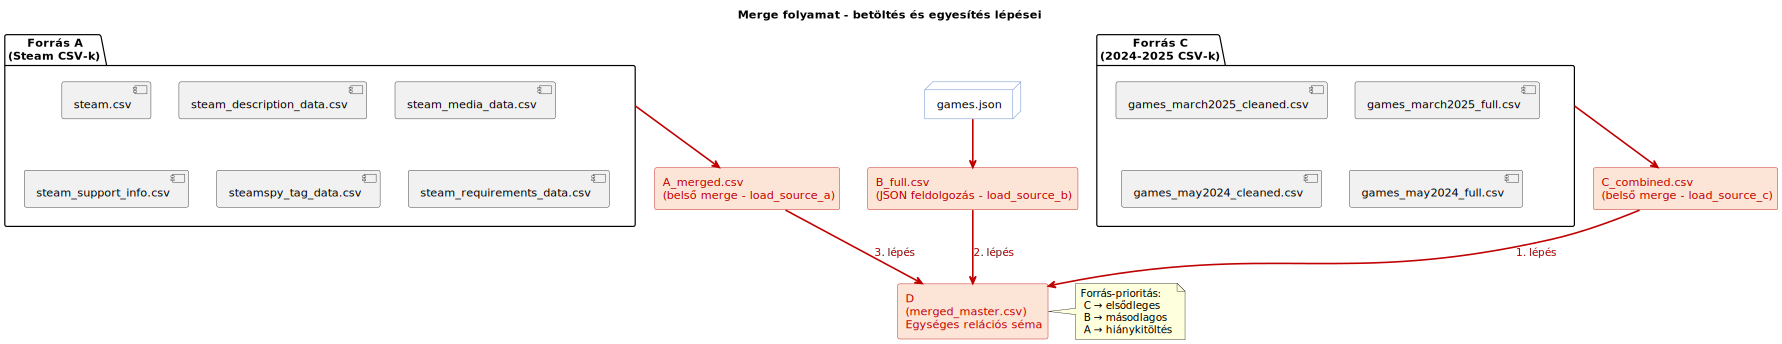
\includegraphics[width=1.0\textwidth]{images/merge_folyamat.pdf}
    \caption{Az A, B és C adathalmazok összefésülésének folyamata}
    \label{fig:merge_process}
\end{figure}


Az ábra PlantUML \cite{plantuml} alapú forráskódja külön fájlban is elérhető (\textit{merge\_process.puml}), amely a folyamat reprodukálhatóságát és dokumentáltságát biztosítja.

\subsubsection{Az összefésülés lépései}

Az \ref{fig:merge_process} ábrán bemutatott folyamat három fő részlépésből áll, amelyek során az egyes forrásadathalmazok önállóan kerülnek feldolgozásra és előkészítésre az egységesítés előtt.

Első lépésként a C forrás feldolgozása történik meg, amely során a 2024-es és 2025-ös CSV-fájlok kerülnek összevonásra és előtisztításra. Ennek eredményeként jön létre a \textit{C\_combined.csv} állomány, amely már egységes szerkezetben tartalmazza az időben eltérő adatforrások adatait.

Második lépésként a B forrás feldolgozása következik, ahol a JSON formátumban elérhető SteamSpy \cite{steamspy} adatok normalizálása és táblásítása történik meg. A feldolgozás eredményeként a \textit{B\_full.csv} állomány jön létre, amely strukturált formában tartalmazza a másodlagos adatforrásból származó információkat.

Harmadik lépésként az A forrás feldolgozása valósul meg, amely során a több CSV-fájlból álló Steam-metaadatok \cite{steam} belső összevonása történik meg. Az eredmény az \textit{A\_merged.csv} állomány, amely az A adathalmaz egységesített változatát tartalmazza.

\subsubsection{Források egyesítése és prioritási sorrend}

Az előfeldolgozott részadathalmazok ezt követően egyesítésre kerülnek egy közös adatállományba. Az összefésülés során meghatározott prioritási sorrend biztosítja, hogy az eltérő források közötti átfedések esetén a legaktuálisabb és legmegbízhatóbb adatok kerüljenek felhasználásra.

A prioritási sorrend az alábbiak szerint alakult:
\begin{itemize}
    \item a C adathalmaz elsődleges forrásként szolgált,
    \item a B adathalmaz másodlagos forrásként került bevonásra,
    \item az A adathalmaz kiegészítő, kitöltő szerepet töltött be.
\end{itemize}

A folyamat eredményeként egy egységes relációs struktúra jött létre (\textit{merged\_master.csv}), amely már közvetlenül alkalmas volt a normalizálási lépések végrehajtására és az SQL-alapú adatbázis felépítésére.

\subsection{Az összefésülés megvalósítása}

Ebben az alfejezetben az A, B és C adathalmazok összefésülésének szoftveres megvalósítása kerül bemutatásra. A merge-folyamat egy moduláris felépítésű Python \cite{python} projektként valósult meg, amely külön kezeli a forrásadatok betöltését, az előfeldolgozási és tisztítási lépéseket, valamint az adatok egységesítését és ellenőrzését. A bemutatott kódrészletek nem a teljes implementációt fedik le, hanem a összefésülés-folyamat szempontjából lényeges, nem triviális megoldásokat szemléltetik.

\subsubsection{A merge-kód felépítése}

Az adathalmazok összefésülésében az alábbi főbb modulok vesznek részt:

\begin{itemize}
    \item \texttt{merge/sources} – az A, B és C forrásadatok beolvasásáért és előtisztításáért felelős modulok,
    \item \texttt{merge/utils} – általános segédfüggvények az adatkezelési, tisztítási, normalizálási és merge-lépések támogatására,
    \item \texttt{merge/visualization} – a mergelt adathalmazra épülő statisztikai ábrák és összefoglaló vizualizációk generálása,
    \item \texttt{merge/output} – a futtatás során keletkező kimeneti állományok és ábrák gyűjtőmappája.
\end{itemize}

A teljes merge-folyamatot a \texttt{merge/main.ipynb} Jupyter \cite{jupyter} munkafüzet vezérli, míg a globális beállításokat és paramétereket a \texttt{merge/config.py} konfigurációs állomány tartalmazza.

\subsubsection{Kiemelt kódrészletek}

A teljes kódbázis részletes ismertetése nem szükséges, ezért az alábbiakban csak néhány olyan megoldás kerül bemutatásra, amelyek jól szemléltetik az összefésülés során alkalmazott logikai döntéseket és adatkezelési stratégiákat. A projekt minden modulja és függvénye részletes dokumentációval (docstringekkel) van ellátva.

\paragraph{Hiányzó adatok kitöltése forrásprioritás alapján}

A merge egyik kulcseleme egy olyan függvény (\ref{lst:missing}), amely a céladatkészlet hiányzó mezőit más forrásokból pótolja. A kitöltés az \textit{appid} alapján történik, és kizárólag azokat az oszlopokat érinti, amelyek mindkét adathalmazban megtalálhatók. A megoldás biztosítja, hogy a források közötti prioritás (C → B → A) ütközésmentesen érvényesüljön.

\begin{python}[caption={Hiányzó adatok pótlása},captionpos=b,label={lst:missing}]
def fill_missing_from_source(d: pd.DataFrame,
                             src: pd.DataFrame) -> pd.DataFrame:
    src = src.copy()
    src["appid"] = src["appid"].astype(str)

    common_cols = [col for col in src.columns if col in d.columns]

    merged = d.merge(
        src[common_cols],
        on="appid",
        how="left",
        suffixes=("", "_src")
    )

    for col in common_cols:
        if col != "appid":
            merged[col] = merged[col].combine_first(merged[f"{col}_src"])
            merged.drop(columns=[f"{col}_src"], inplace=True)

    return merged
\end{python}

\paragraph{Listaértékű attribútumok egyesítése}

A címkék, műfajok, kategóriák és platformok esetében gyakori volt, hogy ugyanazon játékhoz több forrásból is listaértékű adatok tartoztak. Ezek összevonására egy deduplikáló segédfüggvény (\ref{lst:dedup}) került alkalmazásra, amely a különböző forrásokból származó listákat egyesíti, miközben az ismétlődő elemeket eltávolítja.

\begin{python}[caption={Deduplikáló segédfüggvény},captionpos=b,label={lst:dedup}]
def dedup_join(*lists):
    combined = []
    for lst in lists:
        if isinstance(lst, list):
            combined.extend(lst)
    return list(dict.fromkeys(combined))
\end{python}

\paragraph{Képernyőképek több forrásból történő kombinálása}

A képernyőképek kezelése során az A, B és C adathalmazokból származó adatok egyesítése index-alapú leképezéssel történt. A megoldás lehetővé tette, hogy a különböző forrásokból származó képernyőképek a prioritási sorrendnek megfelelően kerüljenek összefűzésre, miközben az egységes attribútumstruktúra megmaradt.

\paragraph{Nyelvi mezők többlépcsős tisztítása}

A nyelvi mezők feldolgozása az egyik legösszetettebb lépés volt, mivel az A, B és C forrásokban eltérő, gyakran zajos formátumban jelentek meg. A normalizálás két egymásra épülő tisztítási lépésből állt: az első lépés a nyers adatok egységesítését és alapvető tisztítását végezte el, míg a második lépés a nyelvnevek szabványosítását és a kontextusfüggő hibák kiszűrését valósította meg. A folyamat eredményeként egy konzisztens, relációs adatbázisba illeszthető nyelvlista jött létre.

\paragraph{A B forrás JSON állományainak feldolgozása}

A B adathalmaz JSON formátumú, beágyazott szerkezete miatt külön betöltési és feldolgozási logika készült. A feldolgozás során az egyes játékokhoz tartozó mezők strukturált rekordokká alakultak, a listaértékű attribútumok normalizált formában kerültek eltárolásra, majd az adatok egységes Pandas DataFrame struktúrába rendeződtek. A feldolgozás fő lépéseit a \ref{lst:b} kódrészlet mutatja be.

\begin{python}[caption={B adathalmaz feldolgozása},captionpos=b,label={lst:b}]
def load_source_b(base_path: str) -> pd.DataFrame:
    file_path = os.path.join(base_path, "games.json")
    with open(file_path, "r", encoding="utf-8") as f:
        dataset = json.load(f)

    records = []
    for appID, game in dataset.items():
        fields = ["name", "release_date", "estimated_owners", "price"]
        record = {key: game.get(key) for key in fields}
        record["appid"] = str(appID)

        list_fields = ["packages", "developers", "publishers", "genres"]
        record.update({f: game.get(f, []) for f in list_fields})

        tags = game.get("tags", {})
        record["tags"] = tags if isinstance(tags, dict) else {}

        records.append(record)

    df_b = pd.DataFrame(records)
    df_b["release_date"] = pd.to_datetime(df_b["release_date"], 
    errors="coerce")
\end{python}

\subsubsection{Logolás és ellenőrzés a merge folyamat során}

Az összefésülési folyamat teljes egészében részletes naplózással került végrehajtásra. A logolás lehetővé tette a forrásfájlok betöltésének, a feldolgozott rekordok számának, valamint az egyes tisztítási és összefésülési lépések nyomon követését. A naplóállományok segítségével a teljes feldolgozási folyamat visszakövethetővé vált, és az esetleges hibák vagy inkonzisztenciák gyorsan azonosíthatók voltak. 

Az összefésülési folyamat során keletkező naplóbejegyzések egy különálló logfájlba kerülnek mentésre. A részletes futási információk, figyelmeztetések és státuszüzenetek a \texttt{merge/merge\_log.txt} állományban kerülnek rögzítésre, amely lehetővé teszi a feldolgozási lépések utólagos ellenőrzését és visszakövetését.


A logolás kiterjedt többek között a forrásadatok betöltésére, az ideiglenes rész-adathalmazok mentésére, az adatok egyesítésére, valamint a végső, egységes D adathalmaz előállítására. Ez a megközelítés biztosította a merge-folyamat átláthatóságát és reprodukálhatóságát.

\Section{Az egységesített adathalmaz felbontása}

Az összefésülési folyamat eredményeként létrejött \textit{merged\_master.csv} egyetlen, nagyméretű, összevont adatállományt tartalmazott. A split folyamat célja az volt, hogy ebből az egységesített táblából tematikus, normalizált CSV-fájlok jöjjenek létre, amelyek közvetlenül megfelelnek a kialakított relációs adatmodell struktúrájának.

A feldolgozás során minden egyes résztábla létrehozása külön függvények segítségével történt. Az elkészült CSV-fájlok a \texttt{split/} könyvtárba kerültek mentésre. A kód futása közben részletes naplózás készült, amely a \texttt{split\_log.txt} állományban rögzíti a feldolgozás egyes lépéseit, biztosítva a folyamat átláthatóságát és visszakövethetőségét.

\subsection{A split folyamat lépései}

A teljes felosztási folyamatot a \texttt{main()} függvény automatizálja, amely az alábbi fő lépésekből áll:
\begin{itemize}
    \item a \textit{merged\_master.csv} állomány betöltése,
    \item az egyes relációknak megfelelő résztáblák létrehozása,
    \item a generált táblák mentése CSV formátumban,
    \item a folyamat közben a feldolgozási lépések naplózása.
\end{itemize}

\subsection{A létrehozott táblák}

A split folyamat során az alábbi CSV-fájlok kerülnek előállításra:
\begin{itemize}
    \item \textit{game.csv} – a videojátékok alapadatai,
    \item \textit{description.csv} – részletes, rövid és „about” leírások,
    \item \textit{media.csv} – fejléc- és háttérképek,
    \item \textit{screenshots.csv} – teljes méretű és előnézeti képernyőképek,
    \item \textit{movies.csv} – videók (Full HD, 480p és előnézeti változatok),
    \item \textit{support.csv} – támogatási URL-ek és e-mail címek,
    \item \textit{requirements.csv} – minimum és ajánlott rendszerkövetelmények operációs rendszer szerint,
    \item \textit{platforms.csv} és \textit{game\_platform.csv} – platformok és kapcsolótábla,
    \item \textit{genres.csv} és \textit{game\_genre.csv} – műfajok és kapcsolótábla,
    \item \textit{categories.csv} és \textit{game\_category.csv} – kategóriák és kapcsolótábla,
    \item \textit{packages.csv}, \textit{sub\_package.csv} és \textit{game\_package.csv} – Steam csomagok és kapcsolatok,
    \item \textit{developers.csv} és \textit{game\_developer.csv} – fejlesztők,
    \item \textit{publishers.csv} és \textit{game\_publisher.csv} – kiadók,
    \item \textit{tags.csv} és \textit{game\_tag.csv} – címkék és súlyozásuk,
    \item \textit{languages.csv} – normalizált nyelvlista,
    \item \textit{game\_subtitles.csv} és \textit{game\_audio\_language.csv} – felirat- és hangnyelvek.
\end{itemize}

\subsection{A split folyamat működési elvei}

A résztáblák előállítása során minden feldolgozási lépés azonos alapelveket követett. A master táblából kizárólag az adott relációhoz tartozó oszlopok kerültek kiválasztásra, a listaértékű mezők normalizálása megtörtént, és szükség esetén új azonosítók kerültek generálásra (például műfajok, címkék vagy nyelvek esetében). A több–több kapcsolatok kezelésére minden esetben külön kapcsolótáblák jöttek létre.

A split folyamat eredményeként az eredetileg egyetlen, összevont adatállományból olyan, logikailag elkülönített és normalizált táblák jöttek létre, amelyek teljes mértékben megfelelnek a relációs adatbázis-tervezési elveknek, és közvetlenül alkalmasak SQL-alapú adatbázisba történő importálásra.

